\documentclass[10pt,twoside]{extarticle}
\usepackage{xcolor}
\usepackage{graphicx}
\usepackage{multicol}
\usepackage{background}
\usepackage{adjustbox}
\usepackage{ifoddpage}
\usepackage{fontawesome}
\usepackage{fontspec}
\setmainfont{DejaVu Sans}
\setlength{\lefthyphenmin}{8}
\setlength{\righthyphenmin}{8}

\usepackage[a5paper]{geometry}
\newcommand{\getdefaultbggraphic}{
	\ifdefined\nobackground
	\else
		\checkoddpage
		\ifoddpage
	   		
\includegraphics[trim = 0 3mm 3mm 3mm,clip,width = \paperwidth,height = \paperheight, keepaspectratio]{images/abstractbackground_right.pdf}
		\else
	   		
\includegraphics[trim = 3mm 3mm 0 3mm,clip,width = \paperwidth,height = \paperheight, keepaspectratio]{images/abstractbackground_left.pdf}
		\fi
	\fi
}

\setlength{\parskip}{0em}
\setlength{\parindent}{0em}
\setlength{\columnsep}{0.3cm}
\setlength{\columnseprule}{0.5pt}

\usepackage{fancyhdr}
\fancypagestyle{abstract} {
	\fancyhead[L]{\vspace*{3em}\makeabstractheader}
	\fancyhead[R]{\makeabstractcredits}
	\fancyfoot{}
	\fancyfoot[C]{\makebox[\textwidth][c]{--- {\thepage} ---}}
	\fancyhfoffset[r]{\dimexpr+0.2cm\relax}
	\renewcommand{\headrulewidth}{0pt}
	\renewcommand{\footrulewidth}{0pt}
	\setlength{\headheight}{50pt}
	\backgroundsetup{opacity = 1, scale = 1, angle = 0,
	   contents = {\getdefaultbggraphic}}
}
\fancypagestyle{default} {
	\fancyhead{}
	\fancyhead[L]{\ifdefined\pagetitletext\vspace*{3em}\pagetitle{\pagetitletext}\\\fi}
	\fancyfoot{}
	\fancyfoot[C]{\makebox[\textwidth][c]{--- {\thepage} ---}}
	\renewcommand{\headrulewidth}{0pt}
	\renewcommand{\footrulewidth}{0pt}
	\setlength{\headheight}{50pt}
	\backgroundsetup{opacity = 1, scale = 1, angle = 0,
	   contents = {\getdefaultbggraphic}}
}
\fancypagestyle{nopagenum} {
	\fancyhead{}
	\fancyfoot{}
	\renewcommand{\headrulewidth}{0pt}
	\renewcommand{\footrulewidth}{0pt}
	\setlength{\headheight}{35pt}
}
\fancypagestyle{empty} {
	\fancyhead{}
	\fancyfoot{}
	\renewcommand{\headrulewidth}{0pt}
	\renewcommand{\footrulewidth}{0pt}
	\setlength{\headheight}{0pt}
	\backgroundsetup{contents = {}}
}
\pagestyle{default}

\title{Reverse Engineering Bootcamp BLACKHOODIE 4}
\author{barbie}
\date{\today}

\newcommand{\fullimagepage}[2]{
	\newpage
	\thispagestyle{nopagenum}
	\ifdefined\nobackground
		\backgroundsetup{contents = {}}
		\vspace*{\fill}
		\vspace{-5em}
		\begin{center}#2\end{center}
		\vspace{\fill}
	\else
		\backgroundsetup{opacity = 1, scale = 1, angle = 0,
			contents = {
					\includegraphics[trim = 0 3mm 3mm 3mm,
					width = \paperwidth,
					height = \paperheight, keepaspectratio]
					{images/#1.png}
			}}
		~\vfill
	\fi
	\newpage
	\backgroundsetup{opacity = 1, scale = 1, angle = 0,
	   contents = {\getdefaultbggraphic}}
}

\definecolor{special}{HTML}{bc994b}

\usepackage{shadowtext}
\shadowoffset{2pt}
\shadowcolor{black!5!white}

% ALTERNATING LETTER COLORS from https://tex.stackexchange.com/a/285974
\ExplSyntaxOn
\NewDocumentCommand{\colorstring}{O{special!90!white,special!95!black}+m}{%
  \clist_set:Nn \l_tmpa_clist {#1}%
  \int_zero:N \l_tmpa_int%
  \str_set:Nx \l_tmpa_str {#2}%
  \int_step_inline:nnnn {1} {1} {\str_count:N \l_tmpa_str } {%
    \str_case_x:nnF {\str_item:Nn \l_tmpa_str {##1}} {%
      {\space}{\space}
    }{%
      \int_compare:nNnTF {\l_tmpa_int } < {\clist_count:N \l_tmpa_clist } {
        \int_incr:N \l_tmpa_int
      }{%
        \int_set:Nn \l_tmpa_int {\c_one}
      }
      \textcolor{\clist_item:Nn \l_tmpa_clist {\l_tmpa_int }}{\hspace{-0.43em}\shadowtext{\str_item:Nn \l_tmpa_str {##1}}}
    }
  }
}
\ExplSyntaxOff

\newcommand{\pagetitle}[1]{%
	\shadowcolor{special!25!white}%
	{\LARGE\textbf{\strut{\colorstring{#1}}}}%
	\shadowcolor{black!5!white}%
}

\newcommand{\cancel}[2]{%
    \tikz[baseline=(tocancel.base)]{
        \node[inner sep=0pt,outer sep=0pt] (tocancel) {#1};
        \node[red] at (0,0.66) {#2};
        \draw[line width=1mm, red] (tocancel.south west) -- (tocancel.north east);
    }%
}%

\def\changemargin#1#2{\list{}{\leftmargin#1\rightmargin#2}\item[]}
\let\endchangemargin=\endlist

\newcommand{\makeabstractheader}{
	\pagetitle{\abstracttitle}\\
	{\small\color{black!40!special}{\textbf{\abstractcomment}}}
}
\newcommand{\makeabstractcredits}{
	\adjustbox{scale={0.85}{1}}{\scriptsize{
		\color{black!40!special}{by \textbf{\abstractowner}}
	}}
}

\usepackage[hidelinks]{hyperref}

\begin{document}

\fullimagepage{titlepage}{{\Large Reverse Engineering Bootcamp}\\{\Huge BLACKHOODIE 4}\\{\large https://www.blackhoodie.re \\ \faTwitter Blackhoodie\_RE}}

\newpage

We roll again, Berlin November 16th-18th! 3 tracks of workshops, two introductory ones, one  advanced; one track is me yelling my usual litany, the other two are entirely held by former attendees and will feature topics of their likings. That might or might not include Windows kernel, ARM, car hacking, yada yada, yes we now hack everything, did I mention that? Former BlackHoodies keep blowing my mind with their advances in not only RE but oh so many different areas. I keep on thinking we might in the end indeed change an industry. Speaking of which, you can be part of it. \textbf{BlackHoodie \#4} will again be free, women-only and super challenging. ALSO, we will again have a one day conference before the workshops, cause two days apparently are not enough!\\

\textbf{WHY WOMEN ONLY} \\

Because a girl-to-girl conversation is so much more fruitful than a full classroom with only one or two women hiding in the corners. I’ve done so many things in my life where I was the only girl among X other participants, and I promise I’ve been hiding in the corners more than once.\\

For the gents it might not be that obvious, but it is not easy for young females who haven’t yet found their place in life to walk into a class room, a university lecture, an office or a conference room full of men. Who, generally speaking, very often very well seem to know their place.\\

I’ve had girls in my classes before, hiding and holding back although I am so certain they would have been capable to be so much better than what their final results showed. So yeah this will be women only, for every female should feel welcomed and encouraged to do her best and get the most out of it.\\

\textbf{WHY MORE WOMEN IN LOW-LEVEL TECHNICAL JOBS IN GENERAL}

\begin{itemize}
	\item It’s difficult. Mastering something difficult makes you happy. I want all of you to be happy.
	\item It pays well. While money makes you also happy, what’s more important, it gives you courage and independence.
	\item It keeps you busy. Lots of open job positions globally, even better, believe it or not it is addictive and you might even find yourself a new hobby.
\end{itemize}

\textbf{HARDFACTS}
\begin{itemize}
	\item There won’t be slides, there will be you, and your debugger, only.
	\item Online preparation assignments, 4 of them, over the course of two months prior to the workshop
	\item No fees, no strings attached, all you have to do is get there
\end{itemize}

\textbf{WHY ARE WE DOING THIS}\\

The concept of women-only has no intention of pulling up walls or feeling exclusive, we don’t need special help, don’t need to be prefered by anything or anyone. I repeat, none of us could give less f*** about being granted a single thing based on our gender.\\

Blackhoodie is about creating space in an industry that’s by definition offensive and very competitive, it is a special invitation for talents who wouldn’t otherwise find the courage to start hacking on their own. It is a place, where attendees feel encouraged to grow skills without pressure, where they can be themselves without having to compete.\\

And, it works. BlackHoodie alumnis have gone far beyond all expectations since the workshop series started. They now hack minesweeper into showing where the damn flags are, give talks at international conferences on how to reconstruct C++ class hierarchies with SMT solvers, or how to gain code execution from XSS abusing the Electron framework, they hold workshops on car hacking, on ARM shellcode writing, on Windows kernel shim abuse.\\

They serve on conference review boards, including BlackHat our industry’s prime venue, and are listed on the prestigious Forbes 30under30 list. I kid you not, most of the BlackHoodie attendees haven’t stuck their noses into security research before they joined the bootcamp.\\

Why so successful you wonder? There are plenty of women out there who are ready to kill, but aren’t sure where to begin. BlackHoodie offers an easy start with a complex topic, packaged up with a courage boost and a neat network of contacts in the industry. This package, paired with the incomparable drive of a chronically underestimated minority, gives the ladies superpowers.\\

– Mari0n \\
\faTwitter pinkflawd

\def\pagetitletext{Before The Bootcamp...}
{\large
\begin{changemargin}{1em}{3em}
\begin{itemize}
~\vspace{\fill}\\
\item{}
\item{The weekend is going to be surprisingly exhausting. Make sure to \textbf{keep yourself hydrated} and \textbf{sleep enough!}}
\vspace*{\fill}\\
\item{Also, \textbf{eat enough} during the breaks. The workshops go on for 3-4 hours and it is not certain if there will be a break.}
\vspace*{\fill}\\
\item{\textbf{Bring you own device with admin rights and charger} as you want to get the most from this weekend.}
\vspace*{\fill}\\
\item{Join our \textbf{IRC channel} in freenode - \#blackhoodie. Ask someone of the STAFF for the password.}
\vspace*{\fill}\\
\item{\textbf{Have fun!} Don’t worry if you can't get everything in the first run. Ask, use the breaks to get to know new people and join us for the evening program, if you can!}
\vspace*{\fill}\\
\end{itemize}
\end{changemargin}
}


\newpage
\fullimagepage{section_talks}{{\Huge Conference}}

\newpage
\fullimagepage{section_workshops}{{\Huge Workshops}}
\def\abstracttitle{Introduction to x86 RE}
\def\abstractcomment{Track 1: welcome party}
\def\abstractowner{Mari0n}

\thispagestyle{abstract}

  \textbf{Prerequisites}
  \begin{itemize}
  	\item Computer science background in a sense you understand programming logic, how a processor works and how an operating system works
  	\item A Notebook capable of running at least one virtual machine
  	\item A virtual machine, preferred Win7 32-bit
  	\item Guts :) (It is going to be a lot to learn in a very short time)
  \end{itemize}

  \textbf{No need to have dealt with x86 before}\\

  \textbf{Description:}\\

  In this track you will be introduced to the basics of malware analysis (static and dynamic) and reversing techniques.\\

  Attendees will have to complete 4 homework assignments before the actual bootcamp in November.\\


\newpage
\def\pagetitletext{}

\thispagestyle{empty}

\vspace*{\fill}
\begin{center}\footnotesize
The Blackhoodie brand, abstracts and graphics belong to\\Marion Marschalek and their original owners.\\
~\\
This booklet is a non-profit project made for distribution at the\\Blackhoodie Bootcamp 2018.\\
~\\
Our intent is to help others to enjoy the reverse engineering and other fields in information security and computer science to the fullest.\\We hope you all have an unforgettable experience.\\
~\\
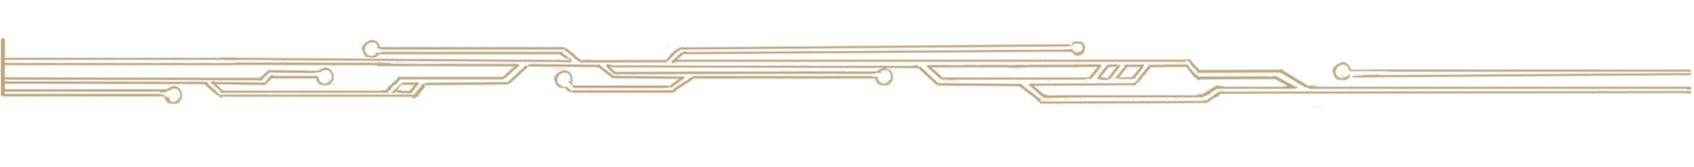
\includegraphics[height=10mm,keepaspectratio]{images/blackhoodie_div.pdf}
\end{center}
\begin{multicols}{3}\footnotesize
\setlength{\columnseprule}{0pt}
\begin{center}
\textbf{Writing}\\barbieauglend\\
~\\
\textbf{Layout and Graphics}\\essy\\
~\\
\textbf{Call for Participation}\\@Blackhoodie\_RE\\Team
\end{center}
\columnbreak
\begin{center}
\textbf{Team Blackhoodie}\\Mari0n\\Bhavna\\Gwaby\\Kylma\\Maria\\Ninon\\Priya\\Thaís\\
\end{center}
\columnbreak
\begin{center}
\textbf{Special Thanks}\\here\\hack.lu\\LaTeX\\And every attendee of the Blackhoodie \#4
\end{center}
\end{multicols}
\vspace{-6em}


\end{document}
